\begin{center}

\includegraphics[width=0.5\textwidth]{content/3/chapter5/images/2.png}\\
Cippi starts the pipeline job
\end{center}

Thanks to the ranges library in C++20, working with the Standard Template Library (STL) is much more comfortable and powerful. The algorithms of the ranges library are lazy, can work directly on containers and can easily be composed. To make it short: The comfort and the power of the ranges library is due to its functional ideas.

Before I dive into the details, here is a first example of the ranges library:

\noindent
Combining the transform and filter functions
\begin{lstlisting}[style=styleCXX]
// rangesFilterTransform.cpp
#include <iostream>
#include <ranges>
#include <vector>
int main() {
	std::vector<int> numbers = {1, 2, 3, 4, 5, 6};
	auto results = numbers | std::views::filter([](int n){ return n % 2 == 0; })
						   | std::views::transform([](int n){ return n * 2; });
	for (auto v: results) std::cout << v << " "; // 4 8 12
}
\end{lstlisting}

You have to read the expression from left to right. The pipe symbol stands for function composition: First, all numbers which are even can pass (std::views::filter([](int n){ return n \% 2 == 0; })). After that, each remaining number is mapped to its double (std::views::transform([](int n){ return n * 2; })). The small example shows two new features of the ranges library: function composition being applied on the entire container.

Now you should be prepared for the details. Let’s go back to square one: ranges and views are concepts.

\subsubsubsection{5.1.1\hspace{0.2cm} The Concepts Ranges and Views}

I already presented the concepts ranges and views in the chapter on concepts. Consequently, here’s a brief refresher.

\begin{itemize}
\item 
range: A range is a group of items that you can iterate over. It provides a begin iterator and an end sentinel. Of course, the containers of the STL are ranges.
\end{itemize}

A view is something that you apply on a range and performs some operation. A view does not own data, and its time complexity to copy, move, or assign is constant.

\noindent
Views operating on a range
\begin{lstlisting}[style=styleCXX]
std::vector<int> numbers = {1, 2, 3, 4, 5, 6};
auto results = numbers | std::views::filter([](int n){ return n % 2 == 0; })
                       | std::views::transform([](int n){ return n * 2; });
\end{lstlisting}

In this code snippet, numbers is the range and std::views::filter and std::views::transform are the views.

Thanks to views, C++20 allows programming in a functional style. Views can be combined and are lazy. I already presented two views, but C++20 offers more.


\begin{center}
Views in C++20
\end{center}

\begin{table}[H]
\centering
\begin{tabular}{ll}
View                                                                                         & Description                                              \\ \hline
\begin{tabular}[c]{@{}l@{}}std::views::all\_t\\ std::views::all\end{tabular}                 & Converts a range into a view.                            \\
std::ranges::ref\_view                                                                       & Takes all elements of another range.                     \\
\begin{tabular}[c]{@{}l@{}}std::ranges::filter\_view\\ std::views::filter\end{tabular}       & Takes the elements that satisfy the predicate.           \\
\begin{tabular}[c]{@{}l@{}}std::ranges::transform\_view\\ std::views::transform\end{tabular} & Transforms each elements.                                \\
\begin{tabular}[c]{@{}l@{}}std::ranges::take\_view\\ std::views::take\end{tabular}           & Takes the first n elements of another view.              \\
\begin{tabular}[c]{@{}l@{}}std::ranges::take\_while\_view\\ std::views::take\_view\end{tabular} &
Takes the elements of another view as long as the preficate returns true. \\
\begin{tabular}[c]{@{}l@{}}std::ranges.drop\_view\\ std::views::drop\end{tabular}            & Skips the first n elements of another view.              \\
\begin{tabular}[c]{@{}l@{}}std::ranges::drop\_while\_view\\ std::views::drop\_while\end{tabular} &
Skips the initial elements of another view until the predicate returns false. \\
\begin{tabular}[c]{@{}l@{}}std::ranges::split\_view\\ std::views::split\end{tabular}         & Splits a view by using a delimiter.                      \\
\begin{tabular}[c]{@{}l@{}}std::ranges::common\_view\\ std::views::common\end{tabular}       & Converts a view into a std::ranges::common\_range.       \\
\begin{tabular}[c]{@{}l@{}}std::ranges::reverse\_view\\ std::views::reverse\end{tabular}     & Iterates in reverse order.                               \\
\begin{tabular}[c]{@{}l@{}}std::ranges::basic\_istream\_view\\ std::ranges::istream\_view\end{tabular} &
Applies operator \textgreater{}\textgreater on the input stream. \\
\begin{tabular}[c]{@{}l@{}}std::ranges::elements\_view\\ std::veiws::elements\end{tabular}   & Creates a view on the n-th element of tuples.            \\
\begin{tabular}[c]{@{}l@{}}std::ranges::keys\_view\\ std::views::keys\end{tabular}           & Creates a view on the first element of pair-like values. \\
\begin{tabular}[c]{@{}l@{}}std::ranges::values\_view\\ std::views::values\end{tabular} &
Creates a view on the second element of pair-like values.
\end{tabular}
\end{table}


In general, you can use a view such as std::views::transform with the alternative name std::ranges:: transform\_view.

\subsubsubsection{5.1.2\hspace{0.2cm} Direct on the Container}

The algorithms of the Standard Template Library (STL) are sometimes a little inconvenient. They need both begin and end iterators. This is often more than you want to write.

\noindent
Algorithms of the STL need both begin and end iterators
\begin{lstlisting}[style=styleCXX]
// sortClassical.cpp

#include <algorithm>
#include <iostream>
#include <vector>

int main() {
	std::vector<int> myVec{-3, 5, 0, 7, -4};
	std::sort(myVec.begin(), myVec.end());
	for (auto v: myVec) std::cout << v << " "; // -4, -3, 0, 5, 7
}
\end{lstlisting}

Wouldn’t it be nice if std::sort could be executed on the entire container? Thanks to the ranges library, this is possible in C++20.

\noindent
Algorithms of the ranges library operate directly on the container
\begin{lstlisting}[style=styleCXX]
// sortRanges.cpp

#include <algorithm>
#include <iostream>
#include <vector>

int main() {
	std::vector<int> myVec{-3, 5, 0, 7, -4};
	std::ranges::sort(myVec);
	for (auto v: myVec) std::cout << v << " "; // -4, -3, 0, 5, 7
}
\end{lstlisting}

Those algorithms of the \href{https://en.cppreference.com/w/cpp/algorithm}{algorithm library}, which are included in the \href{https://en.cppreference.com/w/cpp/header/algorithm}{<algorithm>} header such as std::sort have a ranges pendant std::ranges::sort.

When you study the overloads of std::ranges::sort, you notice that they support a projection.

\noindent
5.1.2.1\hspace{0.2cm} Projection

std::ranges::sort has two overloads:

\noindent
Overload of ‘std::ranges::sort
\begin{lstlisting}[style=styleCXX]
template< std::random_access_iterator I, std::sentinel_for<I> S,
         class Comp = ranges::less, class Proj = std::identity >
requires std::sortable<I, Comp, Proj>
constexpr I sort( I first, S last, Comp comp = {}, Proj proj = {} );

template< ranges::random_access_range R, class Comp = ranges::less,
          class Proj = std::identity >
requires std::sortable<ranges::iterator_t<R>, Comp, Proj>
constexpr ranges::borrowed_iterator_t<R> sort( R&& r, Comp comp = {}, Proj proj = {}\
 );
\end{lstlisting}

When you study the second overload, you notice that it takes a sortable range R, a predicate Comp, and a projection Proj. The predicate Comp uses for default less, and the projection Proj the identity. A projection is a mapping of a set into a subset. Let me show you what that means:

\noindent
Applying projections on data types
\begin{lstlisting}[style=styleCXX]
// rangeProjection.cpp

#include <algorithm>
#include <functional>
#include <iostream>
#include <vector>

struct PhoneBookEntry{
	std::string name;
	int number;
};

void printPhoneBook(const std::vector<PhoneBookEntry>& phoneBook) {
	for (const auto& entry: phoneBook) std::cout << "(" << entry.name << ", "
	                                                    << entry.number << ")";
	std::cout << "\n\n";
}

int main() {
	std::cout << '\n';
	
	std::vector<PhoneBookEntry> phoneBook{ {"Brown", 111}, {"Smith", 444},
		{"Grimm", 666}, {"Butcher", 222}, {"Taylor", 555}, {"Wilson", 333} };
	
	std::ranges::sort(phoneBook, {}, &PhoneBookEntry::name); // ascending by name
	printPhoneBook(phoneBook);
	
	std::ranges::sort(phoneBook, std::ranges::greater() ,
	                  &PhoneBookEntry::name); // descending by name
	printPhoneBook(phoneBook);
	
	std::ranges::sort(phoneBook, {}, &PhoneBookEntry::number); // ascending by number
	printPhoneBook(phoneBook);
	
	std::ranges::sort(phoneBook, std::ranges::greater(),
	                  &PhoneBookEntry::number); // descending by number
	printPhoneBook(phoneBook);
	
	std::cout << '\n';
}
\end{lstlisting}

phoneBook (line 23) has structs of type PhoneBookEntry (line 8). A PhoneBookEntry consists of a name and a number. Thanks to projections, the phoneBook can be sorted in ascending order by name (line 26), descending order by name (line 29), ascending order by number (line 33), and descending order by number (line 36).

\begin{center}
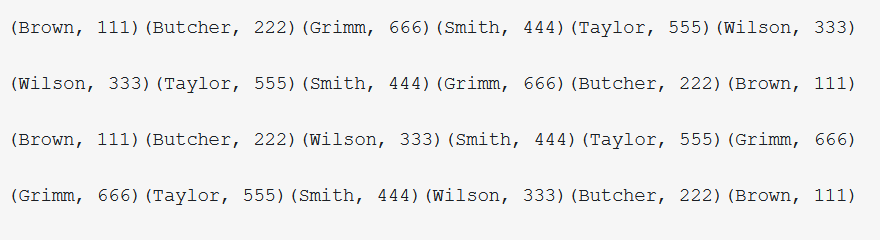
\includegraphics[width=0.8\textwidth]{content/3/chapter5/images/1-1.png}\\
Applying projections on data types
\end{center}

Most ranges algorithms support projections.

\noindent
5.1.2.2\hspace{0.2cm} Direct Views on Keys and Values

Furthermore, you can create direct views on the keys (line 16) and the values (line 24) of a std::unordered\_map.

\noindent
Views on the keys and the values of a std::unordered\_map
\begin{lstlisting}[style=styleCXX]
// rangesEntireContainer.cpp

#include <iostream>
#include <ranges>
#include <string>
#include <unordered_map>

int main() {

std::unordered_map<std::string, int> freqWord{ {"witch", 25}, {"wizard", 33},
												{"tale", 45}, {"dog", 4},
												{"cat", 34}, {"fish", 23} };

	std::cout << "Keys:" << '\n';
	auto names = std::views::keys(freqWord);
	for (const auto& name : names){ std::cout << name << " "; }
	std::cout << '\n';
	for (const auto& name : std::views::keys(freqWord)){ std::cout << name << " "; }
	
	std::cout << "\n\n";

	std::cout << "Values: " << '\n';
	auto values = std::views::values(freqWord);
	for (const auto& value : values){ std::cout << value << " "; }
	std::cout << '\n';
	for (const auto& value : std::views::values(freqWord)) {
		std::cout << value << " ";
	}

}
\end{lstlisting}

Of course, the keys and values can be displayed directly (lines 19 and 27). The output is identical.

\begin{tcblisting}{commandshell={}}
Keys:
fish cat dog tale wizard witch
fish cat dog tale wizard witch

Values:
23 34 4 45 33 25
23 34 4 45 33 25
\end{tcblisting}

\begin{center}
Views on the keys and values of a std::unordered\_map
\end{center}

Working directly on the container might be not so thrilling, but function composition and lazy evaluation are.

\subsubsubsection{5.1.3\hspace{0.2cm} Function Composition}

In the example rangesComposition.cpp, I use a std::map, because the ordering of the keys is crucial.

\noindent
Composition of views
\begin{lstlisting}[style=styleCXX]
// rangesComposition.cpp

#include <iostream>
#include <ranges>
#include <string>
#include <map>

int main() {
	
	std::map<std::string, int> freqWord{ {"witch", 25}, {"wizard", 33},
										{"tale", 45}, {"dog", 4},
										{"cat", 34}, {"fish", 23} };
	
	std::cout << "All words: ";
	for (const auto& name : std::views::keys(freqWord)) { std::cout << name << " "; }
	
	std::cout << '\n';
	
	std::cout << "All words, reverses: ";
	for (const auto& name : std::views::keys(freqWord)
	                      | std::views::reverse) { std::cout << name << " "; }
	
	std::cout << '\n';
	
	std::cout << "The first 4 words: ";
	for (const auto& name : std::views::keys(freqWord)
	                      | std::views::take(4)) { std::cout << name << " "; }
	
	std::cout << '\n';
	
	std::cout << "All words starting with w: ";
	auto firstw = [](const std::string& name){ return name[0] == 'w'; };
	for (const auto& name : std::views::keys(freqWord)
	                      | std::views::filter(firstw)) { std::cout << name << " "; }
	
	std::cout << '\n';

}
\end{lstlisting}

I’m only interested in the keys. I display all of them (line 15), all of them reversed (line 20), the first four (line 26), and the keys starting with the letter ‘w’ (line 32).

Finally, here is the output of the program.

\begin{tcblisting}{commandshell={}}
All words: cat dog fish tale witch wizard
All words, reversed: wizard witch tale fish dog cat
The first 4 words: cat dog fish tale
All words starting with w: witch wizard
\end{tcblisting}

\begin{center}
Composition of views
\end{center}

The pipe symbol | is \href{https://en.wikipedia.org/wiki/Syntactic_sugar}{syntactic sugar} for function composition. Instead of C(R) you can write R | C. Consequently, the next three lines are equivalent.

\noindent
Three syntactic forms of function composition
\begin{lstlisting}[style=styleCXX]
auto rev1 = std::views::reverse(std::views::keys(freqWord));
auto rev2 = std::views::keys(freqWord) | std::views::reverse;
auto rev3 = freqWord | std::views::keys | std::views::reverse;
\end{lstlisting}

\subsubsubsection{5.1.4\hspace{0.2cm} Lazy Evaluation}

std::views::iota is a range factory for creating a sequence of elements by successively incrementing an initial value. This sequence can be finite or infinite. The program rangesIota.cpp fills a std::vector with 10 int’s, starting with 0.

\noindent
Using std::views::iota to fill a std::vector
\begin{lstlisting}[style=styleCXX]
// rangesIota.cpp

#include <iostream>
#include <numeric>
#include <ranges>
#include <vector>

int main() {
	
	std::cout << std::boolalpha;
	
	std::vector<int> vec;
	std::vector<int> vec2;
	
	for (int i: std::views::iota(0, 10)) vec.push_back(i);
	
	for (int i: std::views::iota(0) | std::views::take(10)) vec2.push_back(i);
	
	std::cout << "vec == vec2: " << (vec == vec2) << '\n';
	
	for (int i: vec) std::cout << i << " ";

}
\end{lstlisting}

The first iota call (line 15) creates all numbers from 0 to 9, incremented by 1. The second iota call (line 17) creates an infinite data stream, starting with 0, incremented by 1. std::views::iota(0) is lazy. I only get a new value if I ask for it. I ask for it ten times. Consequently, both vectors are identical.

\begin{tcblisting}{commandshell={}}
vec == vec2: true
0 1 2 3 4 5 6 7 8 9
\end{tcblisting}

\begin{center}
Using std::views::iota to fill a std::vector
\end{center}

Now, I want to solve a small challenge: finding the first 20 prime numbers starting with 1,000,000.

\noindent
The first 20 prime numbers starting with 1’000’000
\begin{lstlisting}[style=styleCXX]
// rangesLazy.cpp

#include <iostream>
#include <ranges>

bool isPrime(int i) {
	for (int j=2; j*j <= i; ++j){
		if (i % j == 0) return false;
	}
	return true;
}

int main() {
	
	std::cout << "Numbers from 1'000'000 to 1'001'000 (displayed each 100th): "
	          << '\n';
	for (int i: std::views::iota(1'000'000, 1'001'000)) {
		if (i % 100 == 0) std::cout << i << " ";
	}
	
	std::cout << "\n\n";
	
	auto odd = [](int i){ return i % 2 == 1; };
	std::cout << "Odd numbers from 1'000'000 to 1'001'000 (displayed each 100th): "
	          << '\n';
	for (int i: std::views::iota(1'000'000, 1'001'000) | std::views::filter(odd)) {
		if (i % 100 == 1) std::cout << i << " ";
	}
	
	std::cout << "\n\n";
	std::cout << "Prime numbers from 1'000'000 to 1'001'000: " << '\n';
	for (int i: std::views::iota(1'000'000, 1'001'000) | std::views::filter(odd)
	                                                   | std::views::filter(isPrime)) {
		std::cout << i << " ";
	}
	
	std::cout << "\n\n";
	
	std::cout << "20 prime numbers starting with 1'000'000: " << '\n';
	for (int i: std::views::iota(1'000'000) | std::views::filter(odd)
	                                        | std::views::filter(isPrime)
	                                        | std::views::take(20)) {
		std::cout << i << " ";
	}
	
	std::cout << '\n';

}
\end{lstlisting}

This is my iterative strategy:

\begin{itemize}
\item 
line 18: Of course, I don’t know when I have 20 primes greater than 1000000. To be on the safe side, I create 1000 numbers. For obvious reasons, I displayed only each 100th.

\item 
line 27: I’m only interested in the odd numbers; therefore, I remove the even numbers.

\item 
line 34: Now, it’s time to apply the next filter. The predicate isPrime (line 7) returns if a number is prime. As you can see in the following screenshot, I was too eager. I got 75 primes.

\item 
line 42: Laziness is a virtue. I use std::iota as an infinite number factory, starting with 1000000 and ask precisely for 20 primes.
\end{itemize}

\begin{center}
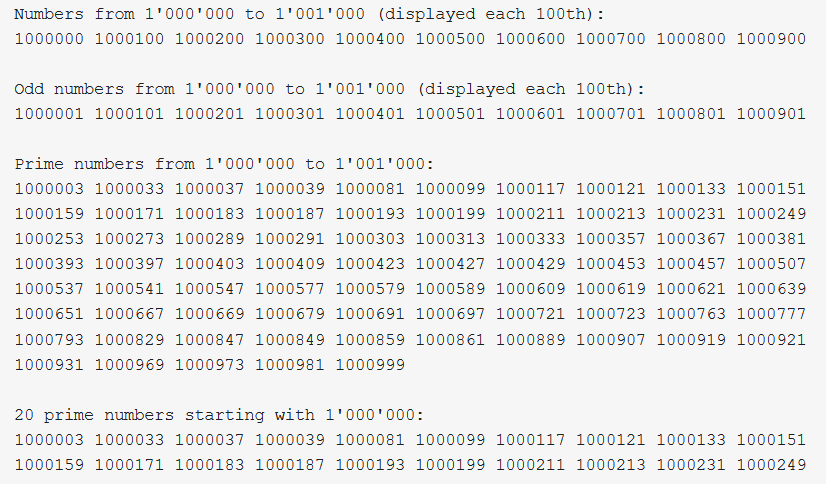
\includegraphics[width=0.6\textwidth]{content/3/chapter5/images/1-2.png}\\
The first 20 prime numbers, starting with 1,000,000
\end{center}

\subsubsubsection{5.1.5\hspace{0.2cm} Define a View}

You can define your own view.

\noindent
5.1.5.1\hspace{0.2cm} std::ranges::view\_interface

Thanks to the \href{https://en.cppreference.com/w/cpp/ranges/view_interface}{std::ranges::view\_interface} helper class, defining a view is easy. To fulfil the concept view, your view needs at least a default constructor, and member functions begin() and end():

\noindent
Your own view
\begin{lstlisting}[style=styleCXX]
class MyView : public std::ranges::view_interface<MyView> {
public:
	auto begin() const { /*...*/ }
	auto end() const { /*...*/ }
};
\end{lstlisting}

By deriving MyView public from the helper class std::ranges::view\_interface using itself as a template parameter, MyView becomes a view. This technique of class template having itself as a template parameter is called \href{https://www.modernescpp.com/index.php/c-is-still-lazy}{Curiously Recurring Template Pattern} (short CRTP).

I use this technique in the next example to create a view out of a container of the Standard Template Library.

\noindent
5.1.5.2\hspace{0.2cm} A Container View

The view ContainerView creates a view on an arbitrary container.

\noindent
Creating a view from a container
\begin{lstlisting}[style=styleCXX]
// containerView.cpp

#include <iostream>
#include <ranges>
#include <string>
#include <vector>

template<std::ranges::input_range Range>
requires std::ranges::view<Range>
class ContainerView : public std::ranges::view_interface<ContainerView<Range>> {
private:
	Range range_{};
	std::ranges::iterator_t<Range> begin_{ std::begin(range_) };
	std::ranges::iterator_t<Range> end_{ std::end(range_) };

public:
	ContainerView() = default;
	
	constexpr ContainerView(Range r): range_(std::move(r)) ,
									begin_(std::begin(r)), end_(std::end(r)) {}
	
	constexpr auto begin() const {
		return begin_;
	}
	constexpr auto end() const {
		return end_;
	}
};

template<typename Range>
ContainerView(Range&& range) -> ContainerView<std::ranges::views::all_t<Range>>;

int main() {

	std::vector<int> myVec{ 1, 2, 3, 4, 5, 6, 7, 8, 9};
	
	auto myContainerView = ContainerView(myVec);
	for (auto c : myContainerView) std::cout << c << " ";
	
	std::cout << '\n';
	
	for (auto i : std::views::reverse(ContainerView(myVec))) std::cout << i << ' ';
	std::cout << '\n';
	
	for (auto i : ContainerView(myVec) | std::views::reverse) std::cout << i << ' ';
	std::cout << '\n';
	
	std::cout << std::endl;
	
	std::string myStr = "Only for testing purpose.";
	
	auto myContainerView2 = ContainerView(myStr);
	for (auto c: myContainerView2) std::cout << c << " ";
	std::cout << '\n';
	
	for (auto i : std::views::reverse(ContainerView(myStr))) std::cout << i << ' ';
	std::cout << '\n';
	
	for (auto i : ContainerView(myStr) | std::views::reverse) std::cout << i << ' ';
	std::cout << '\n';

}
\end{lstlisting}

The class template ContainerView (line 8) derives from the helper class std::ranges::view\_interface and requires that the container support the concept std::ranges::view (line 9). The remaining, minimal implementation is straightforward. ContainerView has a default constructor (line 17), and the two required member functions begin() (line 22) and end() (line 25). For convenience, I added a user-defined deduction guide for class template argument deduction (line 32).

In the main function, I apply the ContainerView on a std::vector (line 37) and a std::string (line 49) and iterate through them forwards and backward.

\begin{center}
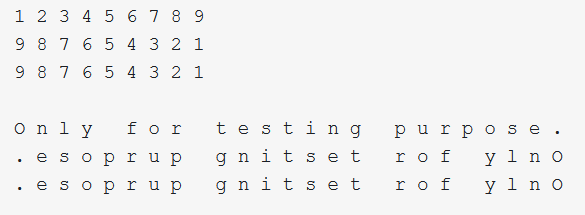
\includegraphics[width=0.6\textwidth]{content/3/chapter5/images/1-3.png}\\
Creating a view from a container
\end{center}

Let me add a few words to the class template argument deduction guide.

\begin{tcolorbox}[colback=blue!5!white,colframe=blue!75!black,title={Class Template Argument Deduction Guide}]
Since C++17, the compiler can deduce template parameters from template arguments. The template deduction guide is a pattern for the compiler to deduce the template arguments.

When you use ContainerView(myVec), the compiler applies the following user-defined deduction guide:

\noindent
User-Defined Deduction Guide for ContainerView
\begin{lstlisting}[style=styleCXX]
template<class Range>
ContainerView(Range&& range) -> ContainerView<std::ranges::views::all_t<Range>>;
\end{lstlisting}

Essentially, a call Container(myVec) causes the compiler to instantiate the code on the right of the arrow ->:

\noindent
Applying the deduction guide for Container(myVec)
\begin{lstlisting}[style=styleCXX]
ContainerView<std::ranges::views::all_t<std::vector<int>&>>(myVec);
\end{lstlisting}

\href{https://en.cppreference.com/w/cpp/language/class_template_argument_deduction}{cppreference.com} provides more information to the user-defined deduction guide for class templates.
\end{tcolorbox}

In the next section on the ranges library, I want to perform a small experiment. Can I add a flavor of Python into C++?

\subsubsubsection{5.1.6\hspace{0.2cm} A Flavor of Python}

The programming language \href{https://www.python.org/}{Python} has the convenient functions filter and map.

\begin{itemize}
\item 
filter: applies a predicate to all elements of an iterable and returns those elements for which the predicate returns true

\item 
map: applies a function to all elements of an iterable and returns a new iterable with the transformed elements
\end{itemize}

An iterable in C++ would be a type that you could use in a range-based for loop.

Furthermore, Python lets you combine both functions in a list comprehension.

\begin{itemize}
\item 
list comprehension: applies a filter and map phase to an iterable and returns a new iterable
\end{itemize}

Here is my challenge: I want to implement Python-like functions filter, map, and list comprehension in C++20 using the ranges library.

\noindent
5.1.6.1\hspace{0.2cm} filter

Python’s filter function can be directly mapped to the corresponding ranges function.

\noindent
Python’s filter function in C++
\begin{lstlisting}[style=styleCXX]
/ filterRanges.cpp

#include <iostream>
 #include <numeric>
 #include <ranges>
 #include <string>
 #include <vector>

template <typename Func, typename Seq>
auto filter(Func func, const Seq& seq) {

	typedef typename Seq::value_type value_type;
	
	std::vector<value_type> result{};
	for (auto i : seq | std::views::filter(func)) result.push_back(i);
	
	return result;
}


int main() {
	
	std::cout << '\n';
	
	std::vector<int> myInts(50);
	std::iota(myInts.begin(), myInts.end(), 1);
	auto res = filter([](int i){ return (i % 3) == 0; }, myInts);
	for (auto v: res) std::cout << v << " ";
	
	
	std::vector<std::string> myStrings{"Only", "for", "testing", "purposes"};
	auto res2 = filter([](const std::string& s){ return std::isupper(s[0]); },
	                       myStrings);
	
	std::cout << "\n\n";
	
	for (auto word: res2) std::cout << word << '\n';
	
	std::cout << '\n';

}
\end{lstlisting}

Before I write a few words about the program, let me show you the output.

\begin{tcblisting}{commandshell={}}
3 6 9 12 15 18 21 24 27 30 33 36 39 42 45 48

Only
\end{tcblisting}

\begin{center}
The filter function applied
\end{center}

The filter function (line 9) should be easy to read. Line 12 detects the type of the underlying element. I just apply the callable func to each element of the sequence and return the elements in the std::vector. Line 27 selects all numbers i from 1 to 50 for which (i \% 3) == 0 holds. Only the strings that start with an uppercase letter can pass the filter in line 32.

\noindent
5.1.6.2\hspace{0.2cm} map

map applies a callable to each element of the input sequence.

\noindent
Python’s map function in C++
\begin{lstlisting}[style=styleCXX]
/ mapRanges.cpp

#include <iostream>
#include <list>
#include <ranges>
#include <string>
#include <vector>
#include <utility>


template <typename Func, typename Seq>
auto map(Func func, const Seq& seq) {

	typedef typename Seq::value_type value_type;
	using return_type = decltype(func(std::declval<value_type>()));
	
	std::vector<return_type> result{};
	for (auto i :seq | std::views::transform(func)) result.push_back(i);
	
	return result;
}

int main() {

	std::cout << '\n';
	
	std::list<int> myInts{1, 2, 3, 4, 5, 6, 7, 8, 9, 10};
	auto res = map([](int i){ return i * i; }, myInts);
	
	for (auto v: res) std::cout << v << " ";
	
	std::cout << "\n\n";
	
	std::vector<std::string> myStrings{"Only", "for", "testing", "purposes"};
	auto res2 = map([](const std::string& s){ return std::make_pair(s.size(), s); },
	                                                                myStrings);
	
	for (auto p: res2) std::cout << "(" << p.first << ", " << p.second << ") " ;
	
	std::cout << "\n\n";

}
\end{lstlisting}

Line 15 in the definition of the map function is quite interesting. The expression decltype(func( std::declval<value\_type>())) deduces the return\_type. The return\_type is the type to which all elements of the input sequence are transformed if the function func is applied to them. std::declval<value\_type>() returns an rvalue reference that decltype can use to deduce the type. This means the call map([](int i){ return i * i; }, myInts) (line 28) maps each element of myInt to its square and the call map([](const std::string\& s){ return std::make\_pair(s.size(), s); }, myStrings) maps each string of myStrings to a pair. The first element of each pair is the length of the string.

\begin{tcblisting}{commandshell={}}
1 4 9 16 25 36 49 64 81 100

(4, Only) (3, for) (7, testing) (8, purposes)
\end{tcblisting}

\begin{center}
The map function applied
\end{center}

\noindent
5.1.6.3\hspace{0.2cm} List Comprehension

The program listComprehensionRanges.cpp has a simplified version of Python’s list-comprehension algorithm.

map applies a callable to each element of the input sequence.

\noindent
A simplified variant of Python’s list comprehension in C++
\begin{lstlisting}[style=styleCXX]
// listComprehensionRanges.cpp

#include <algorithm>
#include <cctype>
#include <functional>
#include <iostream>
#include <ranges>
#include <string>
#include <vector>
#include <utility>

template <typename T>
struct AlwaysTrue {
	constexpr bool operator()(const T&) const {
		return true;
	}
};

template <typename Map, typename Seq, typename Filt = AlwaysTrue<
                                                      typename Seq::value_type>>
auto mapFilter(Map map, Seq seq, Filt filt = Filt()) {

	typedef typename Seq::value_type value_type;
	using return_type = decltype(map(std::declval<value_type>()));
	
	std::vector<return_type> result{};
	for (auto i :seq | std::views::filter(filt)
	                 | std::views::transform(map)) result.push_back(i);
	return result;
}

int main() {

	std::cout << '\n';
	
	std::vector myInts{1, 2, 3, 4, 5, 6, 7, 8, 9, 10};
	
	auto res = mapFilter([](int i){ return i * i; }, myInts);
	for (auto v: res) std::cout << v << " ";
	
	std::cout << "\n\n";
	
	res = mapFilter([](int i){ return i * i; }, myInts,
	[](auto i){ return i % 2 == 1; });
	for (auto v: res) std::cout << v << " ";
	
	std::cout << "\n\n";
	
	std::vector<std::string> myStrings{"Only", "for", "testing", "purposes"};
	auto res2 = mapFilter([](const std::string& s){
	                          return std::make_pair(s.size(), s);
	                       }, myStrings);
	for (auto p: res2) std::cout << "(" << p.first << ", " << p.second << ") " ;
	
	std::cout << "\n\n";
	
	myStrings = {"Only", "for", "testing", "purposes"};
	res2 = mapFilter([](const std::string& s){
	                     return std::make_pair(s.size(), s);
	                 }, myStrings,
	                [](const std::string& word){ return std::isupper(word[0]); });
	
	for (auto p: res2) std::cout << "(" << p.first << ", " << p.second << ") " ;
	
	std::cout << "\n\n";

}
\end{lstlisting}

The default predicate that the filter function applies (line 19) always returns true (line 12). Always true means that the function mapFilter simply behaves by default as a map function. Consequently, the mapFilter function behaves in lines 37 and 49 as does the previous map function. Line 42 and 55 apply both functions map and filter in one call.

\begin{tcblisting}{commandshell={}}
1 4 9 16 25 36 49 64 81 100
	
1 9 25 49 81

(4, Only) (3, for) (7, testing) (8, purposes)

(4, Only)
\end{tcblisting}

\begin{center}
Both functions map and filter applied
\end{center}

\begin{tcolorbox}[colback=mygreen!5!white,colframe=mygreen!75!black,title={Distilled Information}]
\begin{itemize}
\item 
The ranges library provides us with an additional version of the STL algorithms. The ranges library algorithms are lazy, can work directly on containers and can be composed.

\item 
The algorithm of the ranges library
\begin{itemize}
\item 
are lazy and can, therefore, be invoked on infinite data streams.

\item 
can operate directly on the container and don’t need a range defined by two iterators.

\item 
can be composed using the pipe (|) symbol.
\end{itemize}
\end{itemize}
\end{tcolorbox}	
	
	
	
	
	
	
	
	
	
	
	
	
	
	
	
	
	
	
	
	
	
	
	